% -*- mode: Latex; fill-column: 120; -*-
\documentclass{article}\usepackage[]{graphicx}\usepackage[]{color}
%% maxwidth is the original width if it is less than linewidth
%% otherwise use linewidth (to make sure the graphics do not exceed the margin)
\makeatletter
\def\maxwidth{ %
  \ifdim\Gin@nat@width>\linewidth
    \linewidth
  \else
    \Gin@nat@width
  \fi
}
\makeatother

\definecolor{fgcolor}{rgb}{0.345, 0.345, 0.345}
\newcommand{\hlnum}[1]{\textcolor[rgb]{0.686,0.059,0.569}{#1}}%
\newcommand{\hlstr}[1]{\textcolor[rgb]{0.192,0.494,0.8}{#1}}%
\newcommand{\hlcom}[1]{\textcolor[rgb]{0.678,0.584,0.686}{\textit{#1}}}%
\newcommand{\hlopt}[1]{\textcolor[rgb]{0,0,0}{#1}}%
\newcommand{\hlstd}[1]{\textcolor[rgb]{0.345,0.345,0.345}{#1}}%
\newcommand{\hlkwa}[1]{\textcolor[rgb]{0.161,0.373,0.58}{\textbf{#1}}}%
\newcommand{\hlkwb}[1]{\textcolor[rgb]{0.69,0.353,0.396}{#1}}%
\newcommand{\hlkwc}[1]{\textcolor[rgb]{0.333,0.667,0.333}{#1}}%
\newcommand{\hlkwd}[1]{\textcolor[rgb]{0.737,0.353,0.396}{\textbf{#1}}}%
\let\hlipl\hlkwb

\usepackage{framed}
\makeatletter
\newenvironment{kframe}{%
 \def\at@end@of@kframe{}%
 \ifinner\ifhmode%
  \def\at@end@of@kframe{\end{minipage}}%
  \begin{minipage}{\columnwidth}%
 \fi\fi%
 \def\FrameCommand##1{\hskip\@totalleftmargin \hskip-\fboxsep
 \colorbox{shadecolor}{##1}\hskip-\fboxsep
     % There is no \\@totalrightmargin, so:
     \hskip-\linewidth \hskip-\@totalleftmargin \hskip\columnwidth}%
 \MakeFramed {\advance\hsize-\width
   \@totalleftmargin\z@ \linewidth\hsize
   \@setminipage}}%
 {\par\unskip\endMakeFramed%
 \at@end@of@kframe}
\makeatother

\definecolor{shadecolor}{rgb}{.97, .97, .97}
\definecolor{messagecolor}{rgb}{0, 0, 0}
\definecolor{warningcolor}{rgb}{1, 0, 1}
\definecolor{errorcolor}{rgb}{1, 0, 0}
\newenvironment{knitrout}{}{} % an empty environment to be redefined in TeX

\usepackage{alltt}

\usepackage[letterpaper,margin=1in]{geometry}
\usepackage[breaklinks=true,colorlinks=true,urlcolor=blue]{hyperref}
\usepackage{bookmark}
\usepackage{times}
\usepackage{amsmath}
%\usepackage{graphicx}\usepackage[]{color}  knitr adds these
\IfFileExists{upquote.sty}{\usepackage{upquote}}{}
\begin{document}
\title{Fig 2A for paper: Distribution of Chr 1 Deserts\\\large(Chr1, qfiltered)}
\maketitle

\tableofcontents

\section{Intro}
6/1/2017: Simple  script to build fig 2A for the paper, since I can't find Tony's code: distribution of deserts across Chr 1 in all 7 strains.  Some associated investigation of N/NA/gaps in reference sequence.

\section{Preliminaries}
Load utility R code; do setup:
% latex font sizes: \tiny \scriptsize \footnotesize \small \normalsize \large \Large \LARGE \huge \Huge

% setup.my.knitr includes opts_chunk$set(size='footnotesize'), but needed 1st time.
\begin{knitrout}\footnotesize
\definecolor{shadecolor}{rgb}{0.969, 0.969, 0.969}\color{fgcolor}\begin{kframe}
\begin{alltt}
\hlkwd{source}\hlstd{(}\hlstr{'../../../R/wlr.R'}\hlstd{)} \hlcom{# load util code; path relative this folder or sibling in scripts/larrys }
\end{alltt}
\begin{verbatim}
## Running as: ruzzo @ D-10-18-109-56.dhcp4.washington.edu; SVN Id, I miss you.  $Id: wlr.R  2017-07-21 or later $
\end{verbatim}
\begin{alltt}
\hlkwd{setup.my.wd}\hlstd{(}\hlstr{'paperfigs'}\hlstd{)} \hlcom{# set working dir; UPDATE if this file moves, or if COPY/PASTE to new file}
\hlkwd{setup.my.knitr}\hlstd{(}\hlstr{'Fig2A-desert-distribution-figs-knitr/'}\hlstd{)} \hlcom{# knitr's "unnamed-chunk-nnn" figures}
\hlstd{my.figs.dir} \hlkwb{<-} \hlstr{'Fig2A-desert-distribution-figs-mine/'}
\hlkwd{generic.setup}\hlstd{(my.figs.dir)}
\end{alltt}
\end{kframe}
\end{knitrout}
\begin{knitrout}\footnotesize
\definecolor{shadecolor}{rgb}{0.969, 0.969, 0.969}\color{fgcolor}\begin{kframe}
\begin{alltt}
\hlcom{# frequently need to add figpath to file name}
\hlstd{fpath} \hlkwb{<-} \hlkwa{function}\hlstd{(}\hlkwc{base}\hlstd{,} \hlkwc{suffix}\hlstd{=}\hlstr{'.pdf'}\hlstd{,} \hlkwc{dir}\hlstd{=my.figs.dir)\{}
  \hlkwd{return}\hlstd{(}\hlkwd{paste}\hlstd{(dir, base, suffix,} \hlkwc{sep}\hlstd{=}\hlstr{''}\hlstd{))}
\hlstd{\}}
\end{alltt}
\end{kframe}
\end{knitrout}

% latex font sizes: \tiny \scriptsize \footnotesize \small \normalsize \large \Large \LARGE \huge \Huge
\iffalse
\begin{knitrout}\footnotesize
\definecolor{shadecolor}{rgb}{0.969, 0.969, 0.969}\color{fgcolor}\begin{kframe}
\begin{alltt}
\hlcom{# attempt to calibrate print width in footnotesize (this chunk) and scriptsize, tiny (next 2)}
\hlcom{#        1         2         3         4         5         6         7         8         9         A}
\hlcom{#234567890123456789012345678901234567890123456789012345678901234567890123456789012345678901234567890}
\end{alltt}
\end{kframe}
\end{knitrout}

\begin{knitrout}\scriptsize
\definecolor{shadecolor}{rgb}{0.969, 0.969, 0.969}\color{fgcolor}\begin{kframe}
\begin{alltt}
\hlcom{#        1         2         3         4         5         6         7         8         9         A         B}
\hlcom{#2345678901234567890123456789012345678901234567890123456789012345678901234567890123456789012345678901234567890}
\end{alltt}
\end{kframe}
\end{knitrout}

\begin{knitrout}\tiny
\definecolor{shadecolor}{rgb}{0.969, 0.969, 0.969}\color{fgcolor}\begin{kframe}
\begin{alltt}
\hlcom{#        1         2         3         4         5         6         7         8         9         A         B         C         D         E         F         G}
\hlcom{#234567890123456789012345678901234567890123456789012345678901234567890123456789012345678901234567890123456789012345678901234567890123456789012345678901234567890}
\end{alltt}
\end{kframe}
\end{knitrout}
\fi

NOTE: A few code chunks use the knitr cache.  I do NOT check for consistency of cached data with 
code changes and I do NOT know to what extent/whether knitr does, either.  If in doubt, delete
directories ``cache'' (knitr's) and ``00common/mycache'' (mine) to force rebuild.  
%% *TODO* read about knitr cache dependency stuff.

CLEAR CACHE!!!  T/F  will/won't force knitr cache removal (well, actually a rename):

\begin{knitrout}\footnotesize
\definecolor{shadecolor}{rgb}{0.969, 0.969, 0.969}\color{fgcolor}\begin{kframe}
\begin{alltt}
\hlkwd{decache}\hlstd{(}\hlnum{FALSE}\hlstd{)}
\end{alltt}
\begin{verbatim}
# Cache exists, and was left alone.
\end{verbatim}
\end{kframe}
\end{knitrout}

Only using genome seq, so doesn't matter which table set, but qfiltered set is a bit smaller:
\begin{knitrout}\footnotesize
\definecolor{shadecolor}{rgb}{0.969, 0.969, 0.969}\color{fgcolor}\begin{kframe}
\begin{alltt}
\hlcom{# see wlr.R for paths}
\hlstd{snp.tables.chr1q} \hlkwb{<-} \hlkwd{load.snp.tables}\hlstd{(}\hlkwc{use.chr1.tables} \hlstd{=} \hlnum{TRUE} \hlstd{,} \hlkwc{data.name}\hlstd{=}\hlstr{'full.tables.02.25.15'}\hlstd{)}
\end{alltt}
\begin{verbatim}
# Loading ../00common/mycache/snp.tables.chr1.qfiltered.rda ...Loaded.
# Bandaiding qfiltered tables...
\end{verbatim}
\end{kframe}
\end{knitrout}

\begin{knitrout}\footnotesize
\definecolor{shadecolor}{rgb}{0.969, 0.969, 0.969}\color{fgcolor}\begin{kframe}
\begin{alltt}
\hlstd{chr1.len} \hlkwb{<-} \hlkwd{genome.length.constants}\hlstd{()}\hlopt{$}\hlstd{chr1.length}  \hlcom{## 3042585}
\end{alltt}
\end{kframe}
\end{knitrout}

\section{Gaps in the Reference Sequence/SNP Tables}

To place the ``pink'' (gap) bar(s) in the fig, we need to know: How long, how many, where are the gaps in Chr 1 reference sequence?  

\begin{knitrout}\footnotesize
\definecolor{shadecolor}{rgb}{0.969, 0.969, 0.969}\color{fgcolor}\begin{kframe}
\begin{alltt}
\hlcom{# Count 'N's in the ref seq}
\hlstd{ncount} \hlkwb{<-} \hlkwd{unlist}\hlstd{(}\hlkwd{lapply}\hlstd{(snp.tables.chr1q,}\hlkwa{function}\hlstd{(}\hlkwc{x}\hlstd{)} \hlkwd{sum}\hlstd{(x}\hlopt{$}\hlstd{Ref}\hlopt{==}\hlstr{'N'}\hlstd{,}\hlkwc{na.rm}\hlstd{=T)))}
\hlstd{ncount}
\end{alltt}
\begin{verbatim}
# 1007 1012 1013 1014 1015 3367 1335 
#    9   17   16   20   12   16   10
\end{verbatim}
\end{kframe}
\end{knitrout}

\begin{knitrout}\footnotesize
\definecolor{shadecolor}{rgb}{0.969, 0.969, 0.969}\color{fgcolor}\begin{kframe}
\begin{alltt}
\hlcom{# Repeat for NA positions (several columns in the tables are simultaneously NA)}
\hlstd{nacount} \hlkwb{<-} \hlkwa{NULL}
\hlkwa{for}\hlstd{(i} \hlkwa{in} \hlnum{1}\hlopt{:}\hlnum{7}\hlstd{)\{}
  \hlstd{nacount} \hlkwb{<-} \hlkwd{rbind}\hlstd{(nacount,} \hlkwd{unlist}\hlstd{(}\hlkwd{lapply}\hlstd{(snp.tables.chr1q[[i]],}\hlkwa{function}\hlstd{(}\hlkwc{x}\hlstd{)\{}\hlkwd{sum}\hlstd{(}\hlkwd{is.na}\hlstd{(x))\})))}
\hlstd{\}}
\hlkwd{row.names}\hlstd{(nacount)} \hlkwb{<-} \hlkwd{names}\hlstd{(snp.tables.chr1q)}
\hlstd{nacount}
\end{alltt}
\begin{verbatim}
#      snp   Chr   Pos   Ref Cov a g c t n .match exon indel   chr   pos rawCov
# 1007   0 11761 11761 11761   0 0 0 0 0 0      0    0     0 11761 11761      0
# 1012   0 11653 11653 11653   0 0 0 0 0 0      0    0     0 11653 11653      0
# 1013   0 11708 11708 11708   0 0 0 0 0 0      0    0     0 11708 11708      0
# 1014   0 11603 11603 11603   0 0 0 0 0 0      0    0     0 11603 11603      0
# 1015   0 11724 11724 11724   0 0 0 0 0 0      0    0     0 11724 11724      0
# 3367   0 11664 11664 11664   0 0 0 0 0 0      0    0     0 11664 11664      0
# 1335   0 11567 11567 11567   0 0 0 0 0 0      0    0     0 11567 11567      0
\end{verbatim}
\end{kframe}
\end{knitrout}

\begin{knitrout}\footnotesize
\definecolor{shadecolor}{rgb}{0.969, 0.969, 0.969}\color{fgcolor}\begin{kframe}
\begin{alltt}
\hlcom{# Are the NA counts consistent?}
\hlstd{nasummary} \hlkwb{<-} \hlkwd{rbind}\hlstd{(}\hlkwc{max}\hlstd{=}\hlkwd{apply}\hlstd{(nacount,}\hlnum{1}\hlstd{,max),}\hlkwc{min}\hlstd{=}\hlkwd{apply}\hlstd{(nacount[,}\hlkwd{c}\hlstd{(}\hlnum{2}\hlstd{,}\hlnum{3}\hlstd{,}\hlnum{4}\hlstd{,}\hlnum{14}\hlstd{,}\hlnum{15}\hlstd{)],}\hlnum{1}\hlstd{,min))}
\hlstd{nasummary} \hlkwb{<-} \hlkwd{rbind}\hlstd{(nasummary,} \hlkwc{equal}\hlstd{=(nasummary[}\hlnum{1}\hlstd{,]}\hlopt{==}\hlstd{nasummary[}\hlnum{2}\hlstd{,]))}
\hlstd{nasummary}
\end{alltt}
\begin{verbatim}
#        1007  1012  1013  1014  1015  3367  1335
# max   11761 11653 11708 11603 11724 11664 11567
# min   11761 11653 11708 11603 11724 11664 11567
# equal     1     1     1     1     1     1     1
\end{verbatim}
\begin{alltt}
\hlcom{# Consistent? (yes):}
\hlkwd{all}\hlstd{(nasummary[}\hlnum{1}\hlstd{,]}\hlopt{==}\hlstd{nasummary[}\hlnum{2}\hlstd{,])}
\end{alltt}
\begin{verbatim}
# [1] TRUE
\end{verbatim}
\end{kframe}
\end{knitrout}

So, there are 10-20 ``N'' positions in the Chr 1 reference sequence in all 7 isolates and about 11,700 NA positions (with slight variability from strain to strain for each). This variability is seemingly a side effect ofTony's table-build scripts: they leave NA entries where read coverage is zero, which varies a bit, on top of the fixed gap(s) in the reference sequence.  E.g., NA's are sprinkled around, but the only ``N''s are at the edges of the one big gaps.  E.g., note the slightly different placement of the N/NA boundary and the drop in rawCov to zero it corresponding positions here:

\begin{knitrout}\footnotesize
\definecolor{shadecolor}{rgb}{0.969, 0.969, 0.969}\color{fgcolor}\begin{kframe}
\begin{alltt}
\hlstd{snp.tables.chr1q[[}\hlnum{4}\hlstd{]][}\hlnum{358900}\hlopt{:}\hlnum{358915}\hlstd{,]}
\end{alltt}
\begin{verbatim}
#        snp  Chr    Pos  Ref Cov a g c t n .match  exon indel  chr    pos rawCov
# 358900   0 Chr1 358900    T   5 0 0 0 0 0      5 FALSE FALSE Chr1 358900     11
# 358901   0 Chr1 358901    G   3 0 0 1 0 0      2 FALSE FALSE Chr1 358901     10
# 358902   0 Chr1 358902    T   2 0 0 0 0 0      2 FALSE FALSE Chr1 358902      9
# 358903   0 Chr1 358903    N   1 0 0 1 0 0      0 FALSE FALSE Chr1 358903      9
# 358904   0 Chr1 358904    N   1 0 1 0 0 0      0 FALSE FALSE Chr1 358904      8
# 358905   0 Chr1 358905    N   5 0 5 0 0 0      0 FALSE FALSE Chr1 358905      8
# 358906   0 Chr1 358906    N   3 0 3 0 0 0      0 FALSE FALSE Chr1 358906      8
# 358907   0 Chr1 358907    N   0 0 0 0 0 0      0 FALSE FALSE Chr1 358907      7
# 358908   0 Chr1 358908    N   1 1 0 0 0 0      0 FALSE FALSE Chr1 358908      5
# 358909   0 Chr1 358909    N   0 0 0 0 0 0      0 FALSE FALSE Chr1 358909      3
# 358910   0 Chr1 358910    N   1 1 0 0 0 0      0 FALSE FALSE Chr1 358910      1
# 358911   0 Chr1 358911    N   1 0 1 0 0 0      0 FALSE FALSE Chr1 358911      1
# 358912   0 Chr1 358912    N   1 0 0 1 0 0      0 FALSE FALSE Chr1 358912      1
# 358913   0 <NA>     NA <NA>   0 0 0 0 0 0      0 FALSE FALSE <NA>     NA      0
# 358914   0 <NA>     NA <NA>   0 0 0 0 0 0      0 FALSE FALSE <NA>     NA      0
# 358915   0 <NA>     NA <NA>   0 0 0 0 0 0      0 FALSE FALSE <NA>     NA      0
\end{verbatim}
\begin{alltt}
\hlstd{snp.tables.chr1q[[}\hlnum{5}\hlstd{]][}\hlnum{358900}\hlopt{:}\hlnum{358915}\hlstd{,]}
\end{alltt}
\begin{verbatim}
#        snp  Chr    Pos  Ref Cov a g c t n .match  exon indel  chr    pos rawCov
# 358900   0 Chr1 358900    T   1 0 0 0 0 0      1 FALSE FALSE Chr1 358900      3
# 358901   0 Chr1 358901    G   0 0 0 0 0 0      0 FALSE FALSE Chr1 358901      3
# 358902   0 Chr1 358902    T   0 0 0 0 0 0      0 FALSE FALSE Chr1 358902      3
# 358903   0 Chr1 358903    N   0 0 0 0 0 0      0 FALSE FALSE Chr1 358903      2
# 358904   0 Chr1 358904    N   0 0 0 0 0 0      0 FALSE FALSE Chr1 358904      2
# 358905   0 Chr1 358905    N   1 0 1 0 0 0      0 FALSE FALSE Chr1 358905      2
# 358906   0 Chr1 358906    N   1 0 1 0 0 0      0 FALSE FALSE Chr1 358906      2
# 358907   0 Chr1 358907    N   1 1 0 0 0 0      0 FALSE FALSE Chr1 358907      1
# 358908   0 <NA>     NA <NA>   0 0 0 0 0 0      0 FALSE FALSE <NA>     NA      0
# 358909   0 <NA>     NA <NA>   0 0 0 0 0 0      0 FALSE FALSE <NA>     NA      0
# 358910   0 <NA>     NA <NA>   0 0 0 0 0 0      0 FALSE FALSE <NA>     NA      0
# 358911   0 <NA>     NA <NA>   0 0 0 0 0 0      0 FALSE FALSE <NA>     NA      0
# 358912   0 <NA>     NA <NA>   0 0 0 0 0 0      0 FALSE FALSE <NA>     NA      0
# 358913   0 <NA>     NA <NA>   0 0 0 0 0 0      0 FALSE FALSE <NA>     NA      0
# 358914   0 <NA>     NA <NA>   0 0 0 0 0 0      0 FALSE FALSE <NA>     NA      0
# 358915   0 <NA>     NA <NA>   0 0 0 0 0 0      0 FALSE FALSE <NA>     NA      0
\end{verbatim}
\end{kframe}
\end{knitrout}

A position is NA if and only if it has zero coverage, all 7:

\begin{knitrout}\footnotesize
\definecolor{shadecolor}{rgb}{0.969, 0.969, 0.969}\color{fgcolor}\begin{kframe}
\begin{alltt}
\hlstd{na.implies.zero} \hlkwb{<-} \hlkwd{logical}\hlstd{(}\hlnum{7}\hlstd{)}
\hlstd{nonz.implies.nonna} \hlkwb{<-} \hlkwd{logical}\hlstd{(}\hlnum{7}\hlstd{)}
\hlkwa{for}\hlstd{(i} \hlkwa{in} \hlnum{1}\hlopt{:}\hlnum{7}\hlstd{)\{}
  \hlstd{na.implies.zero[i]} \hlkwb{<-} \hlkwd{all}\hlstd{(snp.tables.chr1q[[i]]}\hlopt{$}\hlstd{rawCov[}\hlkwd{is.na}\hlstd{(snp.tables.chr1q[[i]]}\hlopt{$}\hlstd{Ref)]}\hlopt{==}\hlnum{0}\hlstd{)}
  \hlstd{nonz.implies.nonna[i]} \hlkwb{<-} \hlopt{!}\hlkwd{any}\hlstd{(}\hlkwd{is.na}\hlstd{(snp.tables.chr1q[[i]]}\hlopt{$}\hlstd{Ref[snp.tables.chr1q[[i]]}\hlopt{$}\hlstd{rawCov}\hlopt{>}\hlnum{0}\hlstd{]))}
\hlstd{\}}
\hlkwd{all}\hlstd{(na.implies.zero)}
\end{alltt}
\begin{verbatim}
# [1] TRUE
\end{verbatim}
\begin{alltt}
\hlkwd{all}\hlstd{(nonz.implies.nonna)}
\end{alltt}
\begin{verbatim}
# [1] TRUE
\end{verbatim}
\end{kframe}
\end{knitrout}

A closer look.  Here's a representation of positions where one but not all strains show NA; as expected, NA positions show zero coverage; non-NA positions have non-zero coverage, non-NA positions agree on the reference nuc.  

\begin{knitrout}\footnotesize
\definecolor{shadecolor}{rgb}{0.969, 0.969, 0.969}\color{fgcolor}\begin{kframe}
\begin{alltt}
\hlcom{# places where one but not all have NA:}
\hlstd{onena} \hlkwb{<-} \hlkwd{logical}\hlstd{(chr1.len)}
\hlkwa{for} \hlstd{(i} \hlkwa{in} \hlnum{1}\hlopt{:}\hlnum{6}\hlstd{)\{}
  \hlkwa{for}\hlstd{(j} \hlkwa{in} \hlstd{i}\hlopt{:}\hlnum{7}\hlstd{)\{}
    \hlstd{onena} \hlkwb{<-} \hlstd{onena} \hlopt{|} \hlkwd{xor}\hlstd{(}\hlkwd{is.na}\hlstd{(snp.tables.chr1q[[i]]}\hlopt{$}\hlstd{Ref),} \hlkwd{is.na}\hlstd{(snp.tables.chr1q[[j]]}\hlopt{$}\hlstd{Ref))}
  \hlstd{\}}
\hlstd{\}}
\hlstd{nanum1} \hlkwb{<-} \hlkwd{sum}\hlstd{(onena); nanum1}
\end{alltt}
\begin{verbatim}
# [1] 663
\end{verbatim}
\begin{alltt}
\hlcom{# add the few positions that are "N" in all strains (most N's are NA in at least one strain)}
\hlkwa{for}\hlstd{(i} \hlkwa{in} \hlnum{1}\hlopt{:}\hlnum{7}\hlstd{)\{}
  \hlstd{onena[}\hlkwd{which}\hlstd{(snp.tables.chr1q[[i]]}\hlopt{$}\hlstd{Ref} \hlopt{==} \hlstr{'N'}\hlstd{)]} \hlkwb{<-} \hlnum{TRUE}
\hlstd{\}}
\hlstd{nanum2} \hlkwb{<-} \hlkwd{sum}\hlstd{(onena); nanum2}
\end{alltt}
\begin{verbatim}
# [1] 669
\end{verbatim}
\begin{alltt}
\hlcom{# and (for visualization) add a few positions before & after big gap}
\hlstd{onena[}\hlkwd{c}\hlstd{(}\hlnum{358900}\hlopt{:}\hlnum{358902}\hlstd{,}\hlnum{370252}\hlopt{:}\hlnum{370261}\hlstd{)]} \hlkwb{<-} \hlnum{TRUE}
\hlstd{nanum3} \hlkwb{<-} \hlkwd{sum}\hlstd{(onena); nanum3}
\end{alltt}
\begin{verbatim}
# [1] 675
\end{verbatim}
\begin{alltt}
\hlcom{# build a data.frame to display this;}
\hlstd{gapulate} \hlkwb{<-} \hlkwa{function}\hlstd{(}\hlkwc{mask}\hlstd{,} \hlkwc{snp.tab} \hlstd{= snp.tables.chr1q)\{}
  \hlcom{# first, pack ref nucs from all 7 strains together (with '-' for NA)}
  \hlstd{refs} \hlkwb{<-} \hlkwd{character}\hlstd{(}\hlkwd{sum}\hlstd{(mask))}
  \hlkwa{for}\hlstd{(i} \hlkwa{in} \hlnum{1}\hlopt{:}\hlnum{7}\hlstd{)\{}
    \hlstd{tmp} \hlkwb{<-} \hlstd{snp.tab[[i]]}\hlopt{$}\hlstd{Ref[mask]}
    \hlstd{tmp[}\hlkwd{is.na}\hlstd{(tmp)]} \hlkwb{<-} \hlstr{'-'}
    \hlstd{refs} \hlkwb{<-} \hlkwd{paste}\hlstd{(refs, tmp,} \hlkwc{sep}\hlstd{=}\hlstr{''}\hlstd{)}
  \hlstd{\}}
  \hlstd{df.mask} \hlkwb{<-} \hlkwd{data.frame}\hlstd{(}\hlkwc{ref}\hlstd{=refs,} \hlkwc{row.names}\hlstd{=(}\hlnum{1}\hlopt{:}\hlkwd{nrow}\hlstd{(snp.tab[[}\hlnum{1}\hlstd{]]))[mask],} \hlkwc{stringsAsFactors}\hlstd{=F)}
  \hlcom{# then append coverage; zeros turn out to match NAs}
  \hlkwa{for}\hlstd{(i} \hlkwa{in} \hlnum{1}\hlopt{:}\hlnum{7}\hlstd{)\{}
    \hlstd{df.mask} \hlkwb{<-} \hlkwd{cbind}\hlstd{(df.mask, snp.tab[[i]]}\hlopt{$}\hlstd{rawCov[mask])}
    \hlkwd{names}\hlstd{(df.mask)[i}\hlopt{+}\hlnum{1}\hlstd{]} \hlkwb{<-} \hlkwd{names}\hlstd{(snp.tab)[i]}
  \hlstd{\}}
  \hlkwd{return}\hlstd{(df.mask)}
\hlstd{\}}
\hlstd{summary.onena} \hlkwb{<-} \hlkwd{gapulate}\hlstd{(onena)}
\hlcom{# show a few (1st/last few, all N's):}
\hlstd{show.first} \hlkwb{<-} \hlnum{1}\hlopt{:}\hlnum{22}
\hlstd{show.gap}   \hlkwb{<-} \hlkwd{unique}\hlstd{(}\hlkwd{sort}\hlstd{(}\hlkwd{c}\hlstd{(}\hlnum{377}\hlopt{:}\hlnum{404}\hlstd{,}\hlkwd{grep}\hlstd{(}\hlstr{'N'}\hlstd{,summary.onena}\hlopt{$}\hlstd{ref,}\hlkwc{fixed}\hlstd{=T))))}
\hlstd{show.last}  \hlkwb{<-} \hlkwd{nrow}\hlstd{(summary.onena)}\hlopt{+}\hlstd{(}\hlopt{-}\hlnum{5}\hlopt{:}\hlnum{0}\hlstd{)}
\hlstd{summary.onena[show.first,]}  \hlcom{# 1st few}
\end{alltt}
\begin{verbatim}
#           ref 1007 1012 1013 1014 1015 3367 1335
# 1     TTTT-TT    1    1    1    1    0    1    1
# 2     CCCC-CC    3    1    1    1    0    1    1
# 3     CCCC-CC    4    1    1    1    0    1    1
# 4     AAAA-AA    5    1    1    1    0    1    1
# 5     AAAA-AA    7    1    1    1    0    1    1
# 6     GGGG-GG    7    1    1    1    0    1    2
# 7     AAAA-AA   10    1    1    1    0    1    9
# 8     GGGG-GG   12    4    1    1    0    1   11
# 9     TTTT-TT   13    8    1    1    0    1   15
# 10    CCCC-CC   15   10    1    1    0    1   20
# 11    GGGG-GG   16   12    1    1    0    1   22
# 12    AAAA-AA   16   12    1    1    0    1   26
# 13    AAAA-AA   16   15    1    1    0    1   26
# 14    GGGG-GG   17   15    1    1    0    1   28
# 15    TTTT-TT   17   16    1    1    0    1   30
# 16    AAAA-AA   17   16    1    1    0    1   30
# 17    GGGG-GG   17   17    1    1    0    1   33
# 18    TTTT-TT   18   17    1    2    0    1   33
# 19    TTTT-TT   19   18    3    3    0    3   34
# 20    TTTT-TT   20   19    3    3    0    3   35
# 958   AAAAA-A   51   82   36   35   73    0  143
# 20602 TT-TTTT   28   43    0   21   35    1   50
\end{verbatim}
\begin{alltt}
\hlstd{summary.onena[show.gap,]}    \hlcom{# flanks of big gap + all N's}
\end{alltt}
\begin{verbatim}
#            ref 1007 1012 1013 1014 1015 3367 1335
# 358744 T-TTTTT    1    0    1    2    4    4    4
# 358900 TTTTTTT    8   12   13   11    3    9    4
# 358901 GGGGGGG    8   12   13   10    3    9    4
# 358902 TTTTTTT    7   11   12    9    3    9    4
# 358903 NNNNNNN    7   10   10    9    2    8    4
# 358904 NNNNNNN    7    8    9    8    2    5    4
# 358905 NNNNNNN    7    6    5    8    2    3    4
# 358906 NNNNNNN    7    4    3    8    2    3    3
# 358907 NNNNNNN    5    2    3    7    1    3    3
# 358908 NNNN-NN    3    1    3    5    0    3    1
# 358909 NNNN-N-    2    1    3    3    0    1    0
# 358910 N-NN---    1    0    1    1    0    0    0
# 358911 ---N---    0    0    0    1    0    0    0
# 358912 ---N---    0    0    0    1    0    0    0
# 370249 -N-N---    0    1    0    1    0    0    0
# 370250 -N-N-N-    0    2    0    1    0    1    0
# 370251 -NNN-N-    0    2    2    2    0    2    0
# 370252 -NNNNN-    0    3    2    3    1    2    0
# 370253 -NNNNN-    0    3    5    3    1    3    0
# 370254 -NNNNN-    0    3    5    4    1    4    0
# 370255 -NNNNNN    0    3    7    4    2    5    1
# 370256 -NNNNNN    0    6    8    4    2    7    2
# 370257 -NNNNNN    0    8    8    4    3    8    2
# 370258 NNNNNNN    1   11   10    4    5    9    6
# 370259 AAAAAAA    2   12   11    4    5   11   14
# 370260 AAAAAAA    2   13   12    4    7   11   20
# 370261 TTTTTTT    3   15   14    5    7   14   21
# 371397 ----CCC    0    0    0    0    1    4   25
\end{verbatim}
\begin{alltt}
\hlstd{summary.onena[show.last,]}   \hlcom{# last few}
\end{alltt}
\begin{verbatim}
#             ref 1007 1012 1013 1014 1015 3367 1335
# 2993252 --A--AA    0    0    1    0    0    3    6
# 2993253 --GGGGG    0    0    1    1    1    6   10
# 2993254 -AAAAAA    0    4    5    1    2   12   18
# 3042583 AA-AA-A    3    7    0    7    3    0   19
# 3042584 GG-GG-G    3    6    0    7    3    0   17
# 3042585 GG-GG-G    2    4    0    6    2    0   14
\end{verbatim}
\begin{alltt}
\hlstd{chr1.len}
\end{alltt}
\begin{verbatim}
# [1] 3042585
\end{verbatim}
\end{kframe}
\end{knitrout}

Figuring out \emph{where} the gaps are.

\begin{knitrout}\footnotesize
\definecolor{shadecolor}{rgb}{0.969, 0.969, 0.969}\color{fgcolor}\begin{kframe}
\begin{alltt}
\hlstd{make.gap.tab} \hlkwb{<-} \hlkwa{function}\hlstd{(}\hlkwc{nna.mask}\hlstd{,} \hlkwc{snp.tab}\hlstd{=snp.tables.chr1q)\{}
  \hlstd{wna} \hlkwb{<-} \hlkwd{which}\hlstd{(nna.mask)}
  \hlstd{wna} \hlkwb{<-} \hlkwd{append}\hlstd{(wna,wna[}\hlkwd{length}\hlstd{(wna)]}\hlopt{+}\hlnum{999999999}\hlstd{)} \hlcom{#append "infinity"; simplifies end case in loop below}
  \hlcom{#build a table of gaps (i.e., consecutive T's in mask)}
  \hlstd{gap.table} \hlkwb{<-} \hlkwa{NULL}
  \hlstd{g.start.i} \hlkwb{<-} \hlnum{1}
  \hlkwa{for}\hlstd{(i} \hlkwa{in} \hlnum{2}\hlopt{:}\hlkwd{length}\hlstd{(wna))\{}
    \hlkwa{if}\hlstd{(wna[i]}\hlopt{-}\hlstd{wna[i}\hlopt{-}\hlnum{1}\hlstd{]}\hlopt{>}\hlnum{1}\hlstd{)\{}
      \hlstd{g.start} \hlkwb{<-} \hlstd{wna[g.start.i]}
      \hlstd{g.end} \hlkwb{<-} \hlstd{wna[i}\hlopt{-}\hlnum{1}\hlstd{]}
      \hlstd{g.len} \hlkwb{<-} \hlstd{g.end}\hlopt{-}\hlstd{g.start}\hlopt{+}\hlnum{1}
      \hlstd{gap.table} \hlkwb{<-}\hlkwd{rbind}\hlstd{(gap.table,} \hlkwd{c}\hlstd{(}\hlkwc{start}\hlstd{=g.start,} \hlkwc{end}\hlstd{=g.end,} \hlkwc{length}\hlstd{=g.len))}
      \hlstd{g.start.i} \hlkwb{<-} \hlstd{i}
    \hlstd{\}}
  \hlstd{\}}
  \hlkwd{return}\hlstd{(gap.table)}
\hlstd{\}}
\end{alltt}
\end{kframe}
\end{knitrout}
\begin{knitrout}\footnotesize
\definecolor{shadecolor}{rgb}{0.969, 0.969, 0.969}\color{fgcolor}\begin{kframe}
\begin{alltt}
\hlstd{gap.tables} \hlkwb{<-} \hlkwd{vector}\hlstd{(}\hlstr{'list'}\hlstd{,}\hlnum{7}\hlstd{)}
\hlstd{gap.tables2} \hlkwb{<-} \hlkwd{vector}\hlstd{(}\hlstr{'list'}\hlstd{,}\hlnum{7}\hlstd{)}
\hlkwa{for}\hlstd{(st} \hlkwa{in} \hlnum{1}\hlopt{:}\hlnum{7}\hlstd{)\{}
  \hlstd{gap.table} \hlkwb{<-} \hlkwd{make.gap.tab}\hlstd{(}\hlkwd{is.na}\hlstd{(snp.tables.chr1q[[st]]}\hlopt{$}\hlstd{Ref))}
  \hlstd{gap.tables[[st]]} \hlkwb{<-} \hlstd{gap.table}
  \hlcom{# find largest pair of gaps}
  \hlstd{g.max} \hlkwb{<-} \hlkwd{max}\hlstd{(gap.table[,}\hlstr{'length'}\hlstd{])}
  \hlstd{i.max} \hlkwb{<-} \hlkwd{which}\hlstd{(gap.table[,}\hlstr{'length'}\hlstd{]} \hlopt{==} \hlstd{g.max)}
  \hlstd{g.max2} \hlkwb{<-} \hlkwd{max}\hlstd{(gap.table[,}\hlstr{'length'}\hlstd{][}\hlopt{-}\hlstd{i.max])}
  \hlstd{i.max2} \hlkwb{<-} \hlkwd{which}\hlstd{(gap.table[,}\hlstr{'length'}\hlstd{]} \hlopt{==} \hlstd{g.max2)}
  \hlstd{gap.tables2[[st]]} \hlkwb{<-} \hlstd{gap.table[}\hlkwd{c}\hlstd{(i.max,i.max2),]}
\hlstd{\}}
\hlkwd{names}\hlstd{(gap.tables)} \hlkwb{<-} \hlkwd{names}\hlstd{(snp.tables.chr1q)}
\hlcom{#gap.tables}
\hlkwd{names}\hlstd{(gap.tables2)} \hlkwb{<-} \hlkwd{names}\hlstd{(snp.tables.chr1q)}
\hlstd{gap.tables2}
\end{alltt}
\begin{verbatim}
# $`1007`
#       start    end length
# [1,] 358911 370257  11347
# [2,] 149452 149543     92
# 
# $`1012`
#       start    end length
# [1,] 358910 370248  11339
# [2,] 149496 149543     48
# 
# $`1013`
#       start    end length
# [1,] 358911 370250  11340
# [2,] 149478 149536     59
# 
# $`1014`
#       start    end length
# [1,] 358913 370248  11336
# [2,] 149459 149546     88
# 
# $`1015`
#       start    end length
# [1,] 358908 370251  11344
# [2,] 149454 149551     98
# 
# $`3367`
#       start    end length
# [1,] 358910 370249  11340
# [2,] 149478 149527     50
# 
# $`1335`
#       start    end length
# [1,] 358909 370254  11346
# [2,] 149461 149545     85
\end{verbatim}
\end{kframe}
\end{knitrout}

Defining ``gaps'' to be 1 or more consecutive NAs, the chunk above shows (on Chr 1) all 7 isolates have a single gap of about 11340, starting near 358910, while the next largest gap is less that 100 bp.   Based on the earlier look at NA vs N, \emph{none} of the short gaps have N in the ref seq; they just happened to have \emph{coverage} gaps in that strain.  The gap in the ref seq will necessarily have zero counts except at its edges (can't align to NN...N), so what we really want is runs of positions that are NA in all 7, with some border of N's.

\begin{knitrout}\footnotesize
\definecolor{shadecolor}{rgb}{0.969, 0.969, 0.969}\color{fgcolor}\begin{kframe}
\begin{alltt}
\hlstd{nna} \hlkwb{<-} \hlopt{!} \hlkwd{logical}\hlstd{(chr1.len)} \hlcom{#initialize to TRUE}
\hlkwa{for}\hlstd{(i} \hlkwa{in} \hlnum{1}\hlopt{:}\hlnum{7}\hlstd{)\{}
  \hlstd{nna} \hlkwb{<-} \hlstd{nna} \hlopt{&} \hlstd{(}\hlkwd{is.na}\hlstd{(snp.tables.chr1q[[i]]}\hlopt{$}\hlstd{Ref)} \hlopt{|} \hlstd{(snp.tables.chr1q[[i]]}\hlopt{$}\hlstd{Ref}\hlopt{==}\hlstr{'N'}\hlstd{))}
\hlstd{\}}
\hlkwd{sum}\hlstd{(nna)}
\end{alltt}
\begin{verbatim}
# [1] 11469
\end{verbatim}
\begin{alltt}
\hlcom{#there's only one big one:}
\hlstd{all.n.na} \hlkwb{<-} \hlkwd{make.gap.tab}\hlstd{(nna)}
\hlstd{all.n.na}
\end{alltt}
\begin{verbatim}
#         start     end length
#  [1,]  149496  149527     32
#  [2,]  176529  176532      4
#  [3,]  334292  334298      7
#  [4,]  335104  335107      4
#  [5,]  358903  370258  11356
#  [6,]  371402  371426     25
#  [7,]  831869  831877      9
#  [8,] 1416105 1416133     29
#  [9,] 2587051 2587053      3
\end{verbatim}
\begin{alltt}
\hlcom{# and none of the small ones show N's at borders (big gap marked by NNNNNNN @ 358903--370258):}
\hlstd{nnab} \hlkwb{<-} \hlstd{nna}
\hlstd{nnab[}\hlnum{358904}\hlopt{:}\hlnum{370257}\hlstd{]} \hlkwb{<-} \hlnum{FALSE} \hlcom{# omit all but 1st/last of big gap; print rest}
\hlkwd{gapulate}\hlstd{(nnab)}
\end{alltt}
\begin{verbatim}
#             ref 1007 1012 1013 1014 1015 3367 1335
# 149496  -------    0    0    0    0    0    0    0
# 149497  -------    0    0    0    0    0    0    0
# 149498  -------    0    0    0    0    0    0    0
# 149499  -------    0    0    0    0    0    0    0
# 149500  -------    0    0    0    0    0    0    0
# 149501  -------    0    0    0    0    0    0    0
# 149502  -------    0    0    0    0    0    0    0
# 149503  -------    0    0    0    0    0    0    0
# 149504  -------    0    0    0    0    0    0    0
# 149505  -------    0    0    0    0    0    0    0
# 149506  -------    0    0    0    0    0    0    0
# 149507  -------    0    0    0    0    0    0    0
# 149508  -------    0    0    0    0    0    0    0
# 149509  -------    0    0    0    0    0    0    0
# 149510  -------    0    0    0    0    0    0    0
# 149511  -------    0    0    0    0    0    0    0
# 149512  -------    0    0    0    0    0    0    0
# 149513  -------    0    0    0    0    0    0    0
# 149514  -------    0    0    0    0    0    0    0
# 149515  -------    0    0    0    0    0    0    0
# 149516  -------    0    0    0    0    0    0    0
# 149517  -------    0    0    0    0    0    0    0
# 149518  -------    0    0    0    0    0    0    0
# 149519  -------    0    0    0    0    0    0    0
# 149520  -------    0    0    0    0    0    0    0
# 149521  -------    0    0    0    0    0    0    0
# 149522  -------    0    0    0    0    0    0    0
# 149523  -------    0    0    0    0    0    0    0
# 149524  -------    0    0    0    0    0    0    0
# 149525  -------    0    0    0    0    0    0    0
# 149526  -------    0    0    0    0    0    0    0
# 149527  -------    0    0    0    0    0    0    0
# 176529  -------    0    0    0    0    0    0    0
# 176530  -------    0    0    0    0    0    0    0
# 176531  -------    0    0    0    0    0    0    0
# 176532  -------    0    0    0    0    0    0    0
# 334292  -------    0    0    0    0    0    0    0
# 334293  -------    0    0    0    0    0    0    0
# 334294  -------    0    0    0    0    0    0    0
# 334295  -------    0    0    0    0    0    0    0
# 334296  -------    0    0    0    0    0    0    0
# 334297  -------    0    0    0    0    0    0    0
# 334298  -------    0    0    0    0    0    0    0
# 335104  -------    0    0    0    0    0    0    0
# 335105  -------    0    0    0    0    0    0    0
# 335106  -------    0    0    0    0    0    0    0
# 335107  -------    0    0    0    0    0    0    0
# 358903  NNNNNNN    7   10   10    9    2    8    4
# 370258  NNNNNNN    1   11   10    4    5    9    6
# 371402  -------    0    0    0    0    0    0    0
# 371403  -------    0    0    0    0    0    0    0
# 371404  -------    0    0    0    0    0    0    0
# 371405  -------    0    0    0    0    0    0    0
# 371406  -------    0    0    0    0    0    0    0
# 371407  -------    0    0    0    0    0    0    0
# 371408  -------    0    0    0    0    0    0    0
# 371409  -------    0    0    0    0    0    0    0
# 371410  -------    0    0    0    0    0    0    0
# 371411  -------    0    0    0    0    0    0    0
# 371412  -------    0    0    0    0    0    0    0
# 371413  -------    0    0    0    0    0    0    0
# 371414  -------    0    0    0    0    0    0    0
# 371415  -------    0    0    0    0    0    0    0
# 371416  -------    0    0    0    0    0    0    0
# 371417  -------    0    0    0    0    0    0    0
# 371418  -------    0    0    0    0    0    0    0
# 371419  -------    0    0    0    0    0    0    0
# 371420  -------    0    0    0    0    0    0    0
# 371421  -------    0    0    0    0    0    0    0
# 371422  -------    0    0    0    0    0    0    0
# 371423  -------    0    0    0    0    0    0    0
# 371424  -------    0    0    0    0    0    0    0
# 371425  -------    0    0    0    0    0    0    0
# 371426  -------    0    0    0    0    0    0    0
# 831869  -------    0    0    0    0    0    0    0
# 831870  -------    0    0    0    0    0    0    0
# 831871  -------    0    0    0    0    0    0    0
# 831872  -------    0    0    0    0    0    0    0
# 831873  -------    0    0    0    0    0    0    0
# 831874  -------    0    0    0    0    0    0    0
# 831875  -------    0    0    0    0    0    0    0
# 831876  -------    0    0    0    0    0    0    0
# 831877  -------    0    0    0    0    0    0    0
# 1416105 -------    0    0    0    0    0    0    0
# 1416106 -------    0    0    0    0    0    0    0
# 1416107 -------    0    0    0    0    0    0    0
# 1416108 -------    0    0    0    0    0    0    0
# 1416109 -------    0    0    0    0    0    0    0
# 1416110 -------    0    0    0    0    0    0    0
# 1416111 -------    0    0    0    0    0    0    0
# 1416112 -------    0    0    0    0    0    0    0
# 1416113 -------    0    0    0    0    0    0    0
# 1416114 -------    0    0    0    0    0    0    0
# 1416115 -------    0    0    0    0    0    0    0
# 1416116 -------    0    0    0    0    0    0    0
# 1416117 -------    0    0    0    0    0    0    0
# 1416118 -------    0    0    0    0    0    0    0
# 1416119 -------    0    0    0    0    0    0    0
# 1416120 -------    0    0    0    0    0    0    0
# 1416121 -------    0    0    0    0    0    0    0
# 1416122 -------    0    0    0    0    0    0    0
# 1416123 -------    0    0    0    0    0    0    0
# 1416124 -------    0    0    0    0    0    0    0
# 1416125 -------    0    0    0    0    0    0    0
# 1416126 -------    0    0    0    0    0    0    0
# 1416127 -------    0    0    0    0    0    0    0
# 1416128 -------    0    0    0    0    0    0    0
# 1416129 -------    0    0    0    0    0    0    0
# 1416130 -------    0    0    0    0    0    0    0
# 1416131 -------    0    0    0    0    0    0    0
# 1416132 -------    0    0    0    0    0    0    0
# 1416133 -------    0    0    0    0    0    0    0
# 2587051 -------    0    0    0    0    0    0    0
# 2587052 -------    0    0    0    0    0    0    0
# 2587053 -------    0    0    0    0    0    0    0
\end{verbatim}
\begin{alltt}
\hlcom{# so our real gap is:}
\hlstd{the.gap} \hlkwb{<-} \hlstd{all.n.na[}\hlkwd{which}\hlstd{(all.n.na[,}\hlstr{'length'}\hlstd{]}\hlopt{==}\hlkwd{max}\hlstd{(all.n.na[,}\hlstr{'length'}\hlstd{])),]}
\hlstd{the.gap}
\end{alltt}
\begin{verbatim}
#  start    end length 
# 358903 370258  11356
\end{verbatim}
\end{kframe}
\end{knitrout}

\section{Deserts}

Also load the desert tables:

\begin{knitrout}\footnotesize
\definecolor{shadecolor}{rgb}{0.969, 0.969, 0.969}\color{fgcolor}\begin{kframe}
\begin{alltt}
\hlcom{# from svn+ssh://ceg1.ocean.washington.edu/var/svn/7_strains/trunk/code/snpNB/data}
\hlkwd{load}\hlstd{(}\hlstr{'../../../data/des.rda'}\hlstd{)}
\end{alltt}
\end{kframe}
\end{knitrout}

Structure of desert tables:
\begin{knitrout}\footnotesize
\definecolor{shadecolor}{rgb}{0.969, 0.969, 0.969}\color{fgcolor}\begin{kframe}
\begin{alltt}
\hlkwd{names}\hlstd{(des)}         \hlcom{# [1] "tp1007"  "tp1012"  "tp1013"  "tp1014"  "tp1015"  "thapsIT" "tp1335" }
\end{alltt}
\begin{verbatim}
# [1] "tp1007"  "tp1012"  "tp1013"  "tp1014"  "tp1015"  "thapsIT" "tp1335"
\end{verbatim}
\begin{alltt}
\hlkwd{names}\hlstd{(des)[[}\hlnum{6}\hlstd{]]} \hlkwb{<-} \hlstr{'tp3367'}  \hlcom{# override oldschool name}
\hlkwd{names}\hlstd{(des[[}\hlnum{1}\hlstd{]])}    \hlcom{# [1] "Chr1"   ...   "Chr24"}
\end{alltt}
\begin{verbatim}
#  [1] "Chr1"      "Chr2"      "Chr3"      "Chr4"      "Chr5"      "Chr6"      "Chr7"     
#  [8] "Chr8"      "Chr9"      "Chr10"     "Chr11a"    "Chr11b"    "Chr12"     "Chr13"    
# [15] "Chr14"     "Chr15"     "Chr16a"    "Chr16b"    "Chr17"     "Chr18"     "Chr19a_19"
# [22] "Chr19b_31" "Chr19c_29" "Chr20"     "Chr22"     "Chr23"     "Chr24"
\end{verbatim}
\begin{alltt}
\hlkwd{str}\hlstd{(des[[}\hlnum{1}\hlstd{]][[}\hlnum{1}\hlstd{]])}
\end{alltt}
\begin{verbatim}
#  num [1:74, 1:3] 1 8952 19297 91986 211997 ...
#  - attr(*, "dimnames")=List of 2
#   ..$ : NULL
#   ..$ : chr [1:3] "desert origin" "desert terminate" "Length"
\end{verbatim}
\end{kframe}
\end{knitrout}

Show desert containing the gap in all 7:

\begin{knitrout}\footnotesize
\definecolor{shadecolor}{rgb}{0.969, 0.969, 0.969}\color{fgcolor}\begin{kframe}
\begin{alltt}
\hlstd{gapped.desert} \hlkwb{<-} \hlkwd{data.frame}\hlstd{(}\hlkwc{id}\hlstd{=}\hlkwd{names}\hlstd{(des),}\hlkwc{chr}\hlstd{=}\hlstr{'Chr1'}\hlstd{,}\hlkwc{start}\hlstd{=}\hlnum{0}\hlstd{,}\hlkwc{end}\hlstd{=}\hlnum{0}\hlstd{,}\hlkwc{len}\hlstd{=}\hlnum{0}\hlstd{,}\hlkwc{pre.gap}\hlstd{=}\hlnum{0}\hlstd{,}\hlkwc{post.gap}\hlstd{=}\hlnum{0}\hlstd{,}
                            \hlkwc{stringsAsFactors}\hlstd{=}\hlnum{FALSE}\hlstd{)}
\hlkwa{for}\hlstd{(i} \hlkwa{in} \hlnum{1}\hlopt{:}\hlnum{7}\hlstd{)\{}
  \hlstd{hit} \hlkwb{<-} \hlstd{des[[i]][[}\hlnum{1}\hlstd{]][,}\hlnum{1}\hlstd{]} \hlopt{<} \hlstd{the.gap[}\hlstr{'start'}\hlstd{]} \hlopt{&} \hlstd{the.gap[}\hlstr{'end'}\hlstd{]} \hlopt{<}  \hlstd{des[[i]][[}\hlnum{1}\hlstd{]][,}\hlnum{2}\hlstd{]}
  \hlstd{gapped.desert[i,}\hlkwd{c}\hlstd{(}\hlstr{'start'}\hlstd{,}\hlstr{'end'}\hlstd{,}\hlstr{'len'}\hlstd{)]} \hlkwb{<-} \hlstd{des[[i]][[}\hlnum{1}\hlstd{]][hit,]}
\hlstd{\}}
\hlstd{gapped.desert}\hlopt{$}\hlstd{pre.gap}  \hlkwb{<-} \hlstd{the.gap[}\hlstr{'start'}\hlstd{]} \hlopt{-} \hlstd{gapped.desert}\hlopt{$}\hlstd{start}
\hlstd{gapped.desert}\hlopt{$}\hlstd{post.gap} \hlkwb{<-} \hlstd{gapped.desert}\hlopt{$}\hlstd{end} \hlopt{-} \hlstd{the.gap[}\hlstr{'end'}\hlstd{]}
\hlstd{gapped.desert}
\end{alltt}
\begin{verbatim}
#       id  chr  start    end   len pre.gap post.gap
# 1 tp1007 Chr1 332775 371662 38886   26128     1404
# 2 tp1012 Chr1 333012 371708 38695   25891     1450
# 3 tp1013 Chr1 332712 372079 39366   26191     1821
# 4 tp1014 Chr1 331495 371708 40212   27408     1450
# 5 tp1015 Chr1 333127 371708 38580   25776     1450
# 6 tp3367 Chr1 330737 371708 40970   28166     1450
# 7 tp1335 Chr1 332426 371625 39198   26477     1367
\end{verbatim}
\end{kframe}
\end{knitrout}

The post-gap slice of the desert is short enough ($<2$ Kb) that it probably would not qualify as a desert in its own right, but the pre-gap portion ($>25$ Kb) certainly does, and is present in all 7.  From a quick look at the ``big n'' table in ncsnps, it is among the largest of the 7-way shared deserts;  I see only three larger ones ($\approx40$ Kb each, on Chrs 9, 12, and 17).  Fuzzy thought: CNVnator calls 1.5-2.0x coverage for much of the pre-gap region in Italy (but none of the others), making me wonder whether something structural like a mis-assembly, large repeat and/or recombination hotspots may have contributed to the sequencing gap and adjacent desert.  In any case, while a curiosity, it doesn't seem to overturn any of our other interpretation.

\begin{knitrout}\footnotesize
\definecolor{shadecolor}{rgb}{0.969, 0.969, 0.969}\color{fgcolor}\begin{kframe}
\begin{alltt}
\hlkwd{seechunk}\hlstd{(}\hlnum{6}\hlstd{,}\hlnum{350000}\hlstd{,}\hlnum{25000}\hlstd{,}\hlkwc{snp.tables}\hlstd{=snp.tables.chr1q)}
\end{alltt}
\end{kframe}
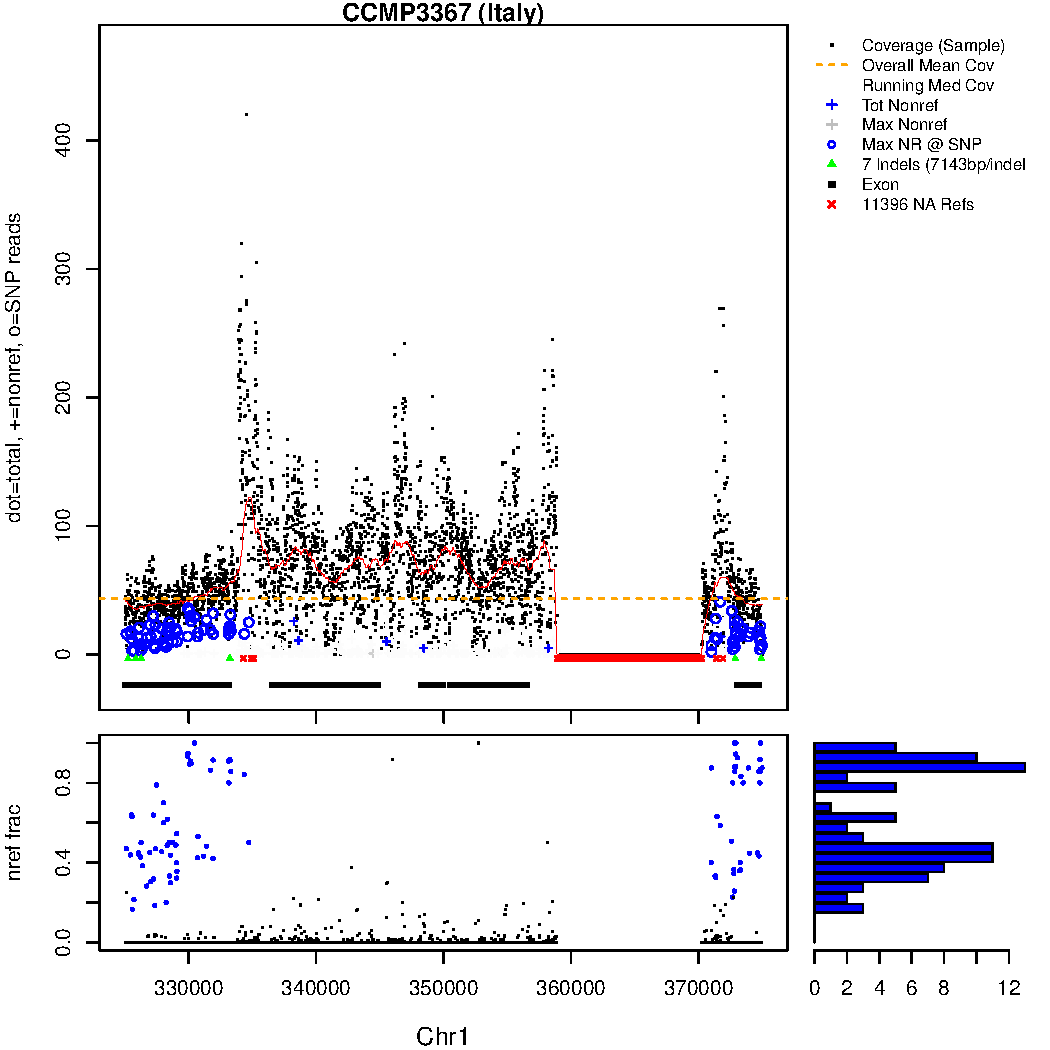
\includegraphics[width=\maxwidth]{Fig2A-desert-distribution-figs-knitr/unnamed-chunk-20-1} 

\end{knitrout}

\section{The Fig}

Order of isolates, top-to-bottom in fig:
\begin{knitrout}\footnotesize
\definecolor{shadecolor}{rgb}{0.969, 0.969, 0.969}\color{fgcolor}\begin{kframe}
\begin{alltt}
\hlstd{strain.order} \hlkwb{<-} \hlkwd{c}\hlstd{(}\hlnum{7}\hlstd{,}\hlnum{1}\hlstd{,}\hlnum{2}\hlstd{,}\hlnum{5}\hlstd{,}\hlnum{4}\hlstd{,}\hlnum{3}\hlstd{,}\hlnum{6}\hlstd{)}
\hlkwd{names}\hlstd{(des)[strain.order]}
\end{alltt}
\begin{verbatim}
# [1] "tp1335" "tp1007" "tp1012" "tp1015" "tp1014" "tp1013" "tp3367"
\end{verbatim}
\end{kframe}
\end{knitrout}

Coordinate system: $x$ coords are genomic positions, i.e., roughly 1..3e6 for Chr 1, printed about 6 inches wide; $y$ coords are arbitrary, think of them as 300 units per inch.  Drawing:  Deserts near each other may visually merge due to the finite size of pixels. To see whether this is distorting the apparent landscape, this code can draw in two modes: first draw each bar as a wide ``nondesert'' (white) rectangle, overlaid by ``desert'' (blue) rectangles for each desert; Optionally, the top half of the bar is the reverse: white nondesert rectangles drawn over a blue background (so non-deserts separated by short deserts may blur together).  This effect is strongest in H-clade where there are many short deserts (shorter than 3Kb, say), but overall I don't think it is misrepresenting the similarities/differences within/between L-/H-clade.  A few sample figures illustrating this are shown below, too.  Additional parameter ``\texttt{min.desert}'' prevents plotting of shorter deserts.

[2017-07-18: write relevant data to Fig2A-data.rda and moved draw.des.row and draw.des.fig to wlr.r so that I can generate Fig2A+B in one script. Various prototyping and exploration left here.]

``Blur'' due to fat pixels.  (Again, botton half draws deserts over white background, then the gap (pink); top half draws non-des over blue background.)

\begin{knitrout}\footnotesize
\definecolor{shadecolor}{rgb}{0.969, 0.969, 0.969}\color{fgcolor}\begin{kframe}
\begin{alltt}
\hlkwd{draw.des.fig}\hlstd{(des, all.n.na,} \hlkwc{draw.nondes}\hlstd{=}\hlnum{TRUE}\hlstd{)}
\end{alltt}
\end{kframe}
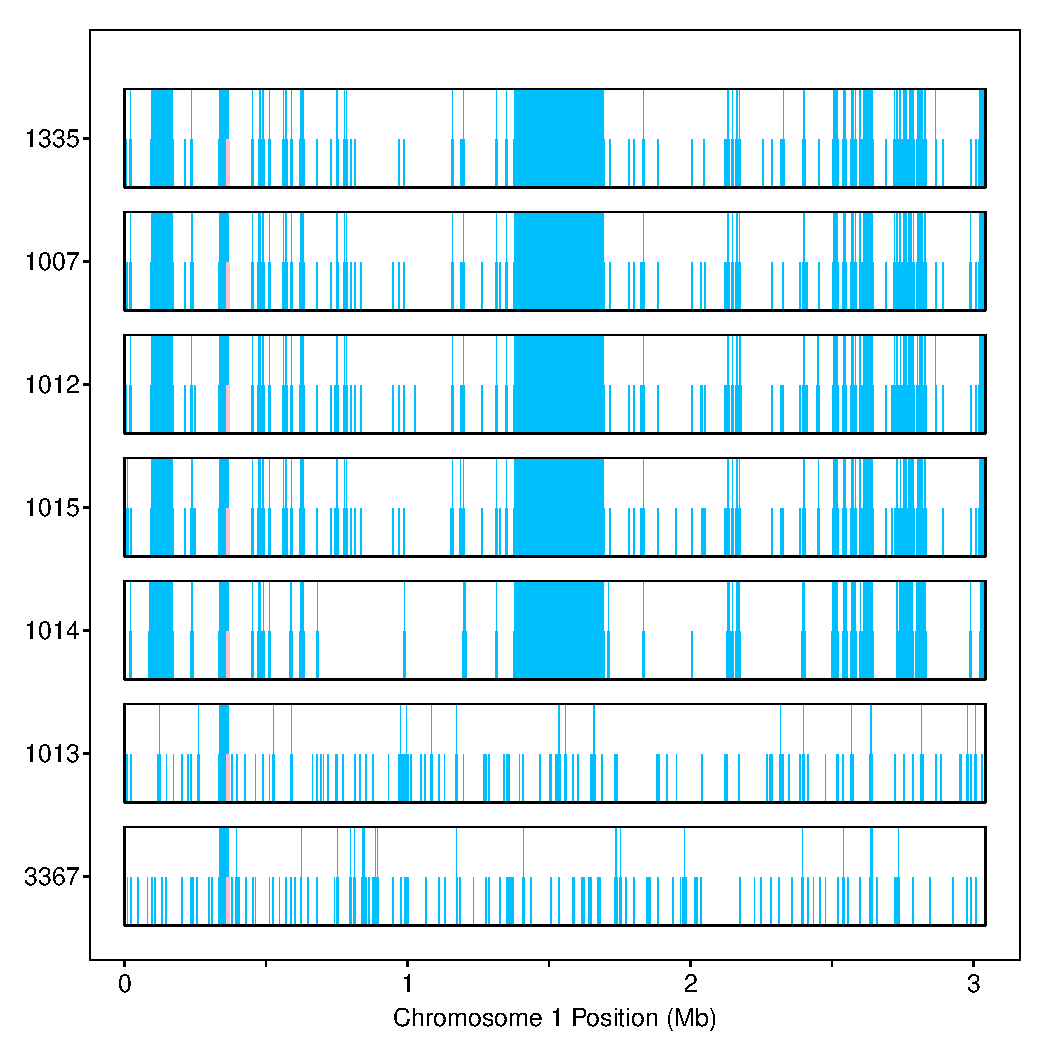
\includegraphics[width=\maxwidth]{Fig2A-desert-distribution-figs-knitr/unnamed-chunk-22-1} 

\end{knitrout}

The effect is slightly ameliorated with short deserts hidden:

\begin{knitrout}\footnotesize
\definecolor{shadecolor}{rgb}{0.969, 0.969, 0.969}\color{fgcolor}\begin{kframe}
\begin{alltt}
\hlkwd{unlist}\hlstd{(}\hlkwd{lapply}\hlstd{(des,}\hlkwa{function}\hlstd{(}\hlkwc{x}\hlstd{)\{}\hlkwd{min}\hlstd{(x[[}\hlnum{1}\hlstd{]][,}\hlstr{'Length'}\hlstd{])\}))}
\end{alltt}
\begin{verbatim}
# tp1007 tp1012 tp1013 tp1014 tp1015 tp3367 tp1335 
#   3503   3389   2106   6330   3222   2348   3676
\end{verbatim}
\begin{alltt}
\hlkwd{draw.des.fig}\hlstd{(des, all.n.na,} \hlkwc{draw.nondes}\hlstd{=}\hlnum{TRUE}\hlstd{,} \hlkwc{min.des}\hlstd{=}\hlnum{3000}\hlstd{)}
\end{alltt}
\end{kframe}
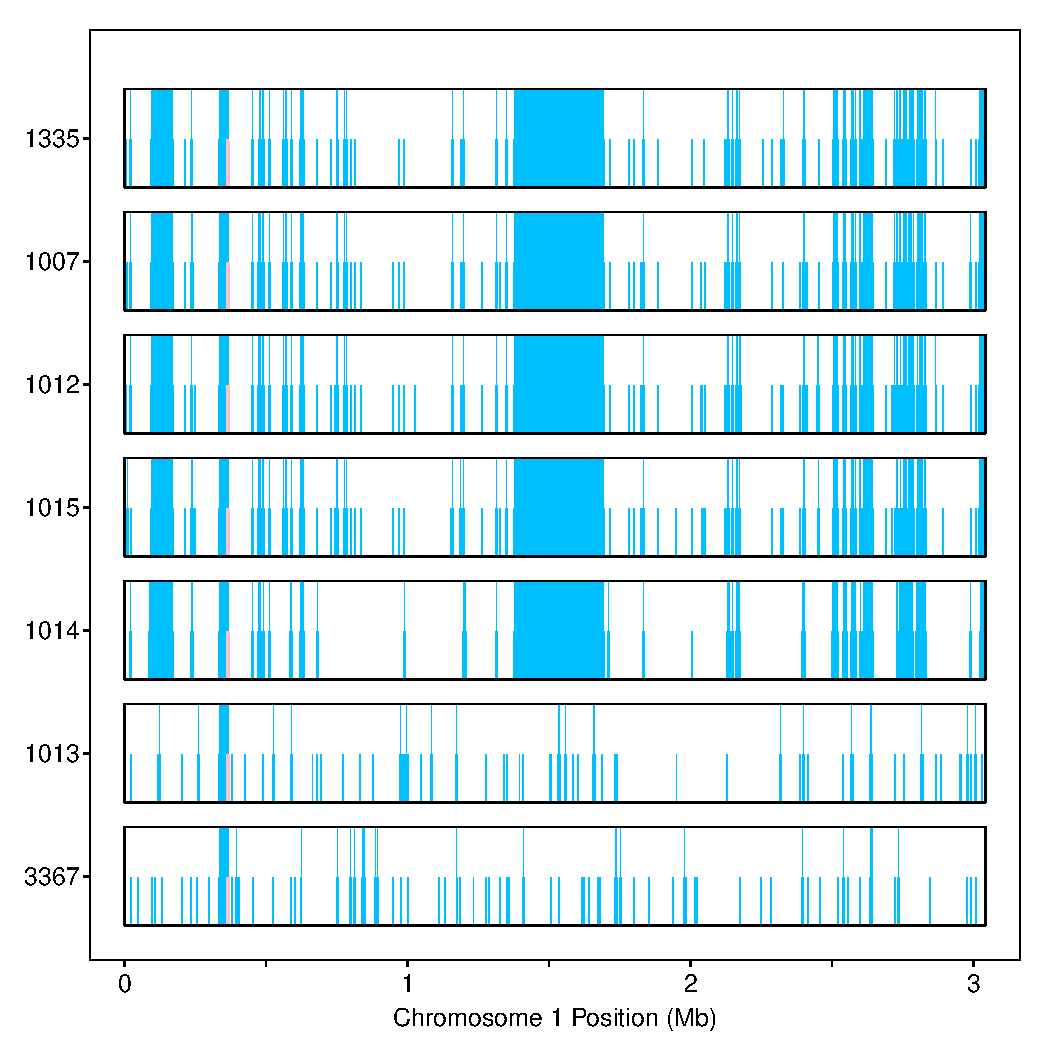
\includegraphics[width=\maxwidth]{Fig2A-desert-distribution-figs-knitr/unnamed-chunk-23-1} 

\end{knitrout}

But, in summary, I think the pixel-blur efect is not so strong that I think we need to deviate from the simple draw-deserts-over-white-background model.
 
Figure prototype for paper:

\begin{knitrout}\footnotesize
\definecolor{shadecolor}{rgb}{0.969, 0.969, 0.969}\color{fgcolor}\begin{kframe}
\begin{alltt}
\hlkwa{if}\hlstd{(}\hlnum{FALSE}\hlstd{)\{}
  \hlcom{# color tests}
  \hlkwd{pdf}\hlstd{(}\hlkwd{fpath}\hlstd{(}\hlstr{'Fig2A-desert-distribution-figa'}\hlstd{),} \hlkwc{width}\hlstd{=}\hlnum{6.5}\hlstd{,} \hlkwc{height}\hlstd{=}\hlnum{3.1}\hlstd{)}
  \hlkwd{draw.des.fig}\hlstd{(des, all.n.na,} \hlkwc{panel.label}\hlstd{=}\hlstr{'A'}\hlstd{,}\hlkwc{gap.col} \hlstd{=} \hlstr{'pink'}\hlstd{)}
  \hlkwd{dev.off}\hlstd{()}
  \hlkwd{pdf}\hlstd{(}\hlkwd{fpath}\hlstd{(}\hlstr{'Fig2A-desert-distribution-figb'}\hlstd{),} \hlkwc{width}\hlstd{=}\hlnum{6.5}\hlstd{,} \hlkwc{height}\hlstd{=}\hlnum{3.1}\hlstd{)}
  \hlkwd{draw.des.fig}\hlstd{(des, all.n.na,} \hlkwc{panel.label}\hlstd{=}\hlstr{'A'}\hlstd{,}\hlkwc{gap.col} \hlstd{=} \hlstr{'deeppink'}\hlstd{)}
  \hlkwd{dev.off}\hlstd{()}
  \hlkwd{pdf}\hlstd{(}\hlkwd{fpath}\hlstd{(}\hlstr{'Fig2A-desert-distribution-figc'}\hlstd{),} \hlkwc{width}\hlstd{=}\hlnum{6.5}\hlstd{,} \hlkwc{height}\hlstd{=}\hlnum{3.1}\hlstd{)}
  \hlkwd{draw.des.fig}\hlstd{(des, all.n.na,} \hlkwc{panel.label}\hlstd{=}\hlstr{'A'}\hlstd{,}\hlkwc{gap.col} \hlstd{=} \hlstr{'goldenrod'}\hlstd{)}
  \hlkwd{dev.off}\hlstd{()}
  \hlkwd{pdf}\hlstd{(}\hlkwd{fpath}\hlstd{(}\hlstr{'Fig2A-desert-distribution-figd'}\hlstd{),} \hlkwc{width}\hlstd{=}\hlnum{6.5}\hlstd{,} \hlkwc{height}\hlstd{=}\hlnum{3.1}\hlstd{)}
  \hlkwd{draw.des.fig}\hlstd{(des, all.n.na,} \hlkwc{panel.label}\hlstd{=}\hlstr{'A'}\hlstd{,}\hlkwc{gap.col} \hlstd{=} \hlstr{'green'}\hlstd{)}
  \hlkwd{dev.off}\hlstd{()}
  \hlkwd{pdf}\hlstd{(}\hlkwd{fpath}\hlstd{(}\hlstr{'Fig2A-desert-distribution-fige'}\hlstd{),} \hlkwc{width}\hlstd{=}\hlnum{6.5}\hlstd{,} \hlkwc{height}\hlstd{=}\hlnum{3.1}\hlstd{)}
  \hlkwd{draw.des.fig}\hlstd{(des, all.n.na,} \hlkwc{panel.label}\hlstd{=}\hlstr{'A'}\hlstd{,}\hlkwc{gap.col} \hlstd{=} \hlstr{'darkgreen'}\hlstd{)}
  \hlkwd{dev.off}\hlstd{()}
  \hlkwd{pdf}\hlstd{(}\hlkwd{fpath}\hlstd{(}\hlstr{'Fig2A-desert-distribution-figf'}\hlstd{),} \hlkwc{width}\hlstd{=}\hlnum{6.5}\hlstd{,} \hlkwc{height}\hlstd{=}\hlnum{3.1}\hlstd{)}
  \hlkwd{draw.des.fig}\hlstd{(des, all.n.na,} \hlkwc{panel.label}\hlstd{=}\hlstr{'A'}\hlstd{,}\hlkwc{gap.col} \hlstd{=} \hlstr{'yellow'}\hlstd{)}
  \hlkwd{dev.off}\hlstd{()}
  \hlkwd{pdf}\hlstd{(}\hlkwd{fpath}\hlstd{(}\hlstr{'Fig2A-desert-distribution-figg'}\hlstd{),} \hlkwc{width}\hlstd{=}\hlnum{6.5}\hlstd{,} \hlkwc{height}\hlstd{=}\hlnum{3.1}\hlstd{)}
  \hlkwd{draw.des.fig}\hlstd{(des, all.n.na,} \hlkwc{panel.label}\hlstd{=}\hlstr{'A'}\hlstd{,}\hlkwc{gap.col} \hlstd{=} \hlstr{'orange'}\hlstd{)}
  \hlkwd{dev.off}\hlstd{()}
  \hlkwd{pdf}\hlstd{(}\hlkwd{fpath}\hlstd{(}\hlstr{'Fig2A-desert-distribution-figh'}\hlstd{),} \hlkwc{width}\hlstd{=}\hlnum{6.5}\hlstd{,} \hlkwc{height}\hlstd{=}\hlnum{3.1}\hlstd{)}
  \hlkwd{draw.des.fig}\hlstd{(des, all.n.na,} \hlkwc{panel.label}\hlstd{=}\hlstr{'A'}\hlstd{,}\hlkwc{gap.col} \hlstd{=} \hlstr{'grey55'}\hlstd{)}
  \hlkwd{dev.off}\hlstd{()}
  \hlkwd{pdf}\hlstd{(}\hlkwd{fpath}\hlstd{(}\hlstr{'Fig2A-desert-distribution-figi'}\hlstd{),} \hlkwc{width}\hlstd{=}\hlnum{6.5}\hlstd{,} \hlkwc{height}\hlstd{=}\hlnum{3.1}\hlstd{)}
  \hlkwd{draw.des.fig}\hlstd{(des, all.n.na,} \hlkwc{panel.label}\hlstd{=}\hlstr{'A'}\hlstd{,}\hlkwc{gap.col} \hlstd{=} \hlstr{'firebrick2'}\hlstd{)}
  \hlkwd{dev.off}\hlstd{()}
  \hlkwd{pdf}\hlstd{(}\hlkwd{fpath}\hlstd{(}\hlstr{'Fig2A-desert-distribution-figj'}\hlstd{),} \hlkwc{width}\hlstd{=}\hlnum{6.5}\hlstd{,} \hlkwc{height}\hlstd{=}\hlnum{3.1}\hlstd{)}
  \hlkwd{draw.des.fig}\hlstd{(des, all.n.na,} \hlkwc{panel.label}\hlstd{=}\hlstr{'A'}\hlstd{,}\hlkwc{gap.col} \hlstd{=} \hlstr{'hotpink'}\hlstd{)}
  \hlkwd{dev.off}\hlstd{()}
  \hlkwd{pdf}\hlstd{(}\hlkwd{fpath}\hlstd{(}\hlstr{'Fig2A-desert-distribution-figk'}\hlstd{),} \hlkwc{width}\hlstd{=}\hlnum{6.5}\hlstd{,} \hlkwc{height}\hlstd{=}\hlnum{3.1}\hlstd{)}
  \hlkwd{draw.des.fig}\hlstd{(des, all.n.na,} \hlkwc{panel.label}\hlstd{=}\hlstr{'A'}\hlstd{,}\hlkwc{gap.col} \hlstd{=} \hlstr{'firebrick3'}\hlstd{)}
  \hlkwd{dev.off}\hlstd{()}
  \hlkwd{pdf}\hlstd{(}\hlkwd{fpath}\hlstd{(}\hlstr{'Fig2A-desert-distribution-figl'}\hlstd{),} \hlkwc{width}\hlstd{=}\hlnum{6.5}\hlstd{,} \hlkwc{height}\hlstd{=}\hlnum{3.1}\hlstd{)}
  \hlkwd{draw.des.fig}\hlstd{(des, all.n.na,} \hlkwc{panel.label}\hlstd{=}\hlstr{'A'}\hlstd{,}\hlkwc{gap.col} \hlstd{=} \hlstr{'grey80'}\hlstd{,}\hlkwc{d.col}\hlstd{=}\hlstr{'dodgerblue2'}\hlstd{)}
  \hlkwd{dev.off}\hlstd{()}
  \hlkwd{pdf}\hlstd{(}\hlkwd{fpath}\hlstd{(}\hlstr{'Fig2A-desert-distribution-figm'}\hlstd{),} \hlkwc{width}\hlstd{=}\hlnum{6.5}\hlstd{,} \hlkwc{height}\hlstd{=}\hlnum{2.1}\hlstd{)}
  \hlkwd{draw.des.fig}\hlstd{(des, all.n.na,} \hlkwc{panel.label}\hlstd{=}\hlstr{'A'}\hlstd{,}\hlkwc{gap.col} \hlstd{=} \hlstr{'gold'}\hlstd{,}\hlkwc{d.col}\hlstd{=}\hlstr{'dodgerblue2'}\hlstd{)}
  \hlkwd{dev.off}\hlstd{()}
  \hlkwd{pdf}\hlstd{(}\hlkwd{fpath}\hlstd{(}\hlstr{'Fig2A-desert-distribution-fign'}\hlstd{),} \hlkwc{width}\hlstd{=}\hlnum{6.5}\hlstd{,} \hlkwc{height}\hlstd{=}\hlnum{2.1}\hlstd{)}
  \hlkwd{draw.des.fig}\hlstd{(des, all.n.na,} \hlkwc{panel.label}\hlstd{=}\hlstr{'A'}\hlstd{,}\hlkwc{gap.col} \hlstd{=} \hlstr{'gold'}\hlstd{,}\hlkwc{d.col}\hlstd{=}\hlstr{'dodgerblue2'}\hlstd{,}\hlkwc{min.des}\hlstd{=}\hlnum{5000}\hlstd{)}
  \hlkwd{dev.off}\hlstd{()}
  \hlkwd{pdf}\hlstd{(}\hlkwd{fpath}\hlstd{(}\hlstr{'Fig2A-desert-distribution-figo'}\hlstd{),} \hlkwc{width}\hlstd{=}\hlnum{6.5}\hlstd{,} \hlkwc{height}\hlstd{=}\hlnum{2.1}\hlstd{)}
  \hlkwd{draw.des.fig}\hlstd{(des, all.n.na,} \hlkwc{panel.label}\hlstd{=}\hlstr{'A'}\hlstd{,}\hlkwc{gap.col} \hlstd{=} \hlstr{'gold'}\hlstd{,}\hlkwc{d.col}\hlstd{=}\hlstr{'dodgerblue2'}\hlstd{,}\hlkwc{min.des}\hlstd{=}\hlnum{8000}\hlstd{)}
  \hlkwd{dev.off}\hlstd{()}
  \hlkwd{pdf}\hlstd{(}\hlkwd{fpath}\hlstd{(}\hlstr{'Fig2A-desert-distribution-figp'}\hlstd{),} \hlkwc{width}\hlstd{=}\hlnum{6.5}\hlstd{,} \hlkwc{height}\hlstd{=}\hlnum{2.1}\hlstd{)}
  \hlkwd{draw.des.fig}\hlstd{(des, all.n.na,} \hlkwc{panel.label}\hlstd{=}\hlstr{'A'}\hlstd{,}\hlkwc{gap.col} \hlstd{=} \hlstr{'gold'}\hlstd{,}\hlkwc{d.col}\hlstd{=}\hlstr{'dodgerblue2'}\hlstd{,}\hlkwc{min.des}\hlstd{=}\hlnum{10000}\hlstd{)}
  \hlkwd{dev.off}\hlstd{()}
\hlstd{\}}
\hlkwd{pdf}\hlstd{(}\hlkwd{fpath}\hlstd{(}\hlstr{'Fig2A-desert-distribution-figq'}\hlstd{),} \hlkwc{width}\hlstd{=}\hlnum{6.5}\hlstd{,} \hlkwc{height}\hlstd{=}\hlnum{2.1}\hlstd{)}
\hlkwd{draw.des.fig}\hlstd{(des, all.n.na,} \hlkwc{panel.label}\hlstd{=}\hlstr{'A'}\hlstd{,}\hlkwc{gap.col} \hlstd{=} \hlstr{'gold'}\hlstd{,}\hlkwc{d.col}\hlstd{=}\hlstr{'dodgerblue2'}\hlstd{,}\hlkwc{min.des}\hlstd{=}\hlnum{10000}\hlstd{,}\hlkwc{twotone}\hlstd{=}\hlstr{'lightblue'}\hlstd{)}
\hlkwd{dev.off}\hlstd{()}
\end{alltt}
\begin{verbatim}
# pdf 
#   2
\end{verbatim}
\end{kframe}
\end{knitrout}
\noindent and shown juxtaposed with Fig2b for comparison as Fig~\ref{fig:2a2b}.  (Surrounding boxes just to make marginal space obvious; change fbox to mbox to remove.)
\\ 3/22/2018: Oh, Fig2B no longer exists separately, since fig2-glue.rnw now builds the full fig 2.
\begin{figure}
  \begin{center}
    \fbox{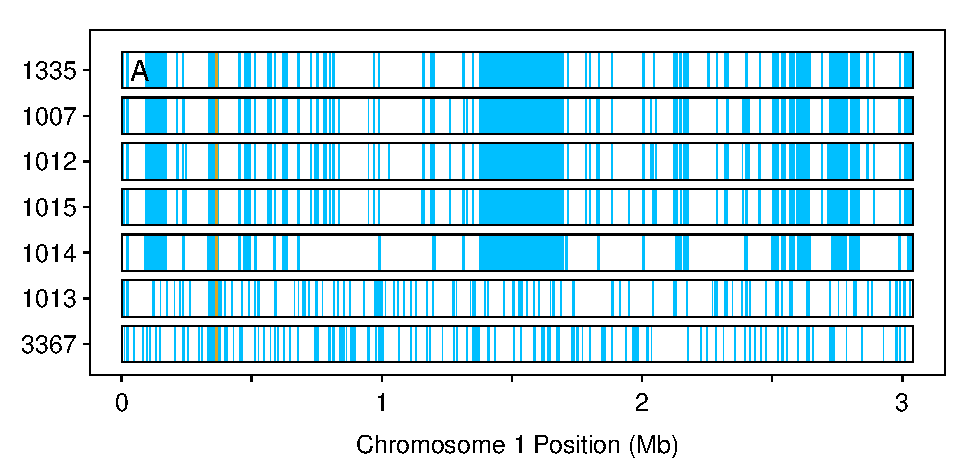
\includegraphics{Fig2A-desert-distribution-figs-mine/Fig2A-desert-distribution-fig.pdf}}\\
    \fbox{[Panel B goes here]}%%%\includegraphics{../../../inst/doc/figures4paper/Fig2B-bigdes-snpdens-ny.pdf}}
  \end{center}
  \caption{Proposed caption: Attributes of SNP deserts for {\it T. pseudonana\/} isolates. A) SNP distributions across the 3 Mb of Chromosome 1 for the seven {\it T. pseudonana\/} isolates. Regions in blue have significantly low SNP density (``SNP deserts'') based on a negative binomial model (Methods). Pink(???) region is a gap of known size in the reference sequence. The large region centered near 1.5Mb is a 320Kb SNP desert present in all L-isolates but neither H-isolate. B) SNP densities (SNP per base-pair---$\mu\pm2\sigma$) in the 29 deserts that span at least 50Kb of the CCMP 1335 genome (blue) and the thirty regions surrounding these deserts (including deserts smaller than 50Kb; black).  }
  \label{fig:2a2b}
\end{figure}

\begin{knitrout}\footnotesize
\definecolor{shadecolor}{rgb}{0.969, 0.969, 0.969}\color{fgcolor}\begin{kframe}
\begin{alltt}
\hlstd{Fig2A.data.Description} \hlkwb{<-} \hlstr{'This .rda file contains the "gap table" all.n.na built by Fig2A-desert-distribution.rnw'}
\hlkwd{save}\hlstd{(Fig2A.data.Description, all.n.na,}\hlkwc{file}\hlstd{=}\hlstr{'Fig2A-data.rda'}\hlstd{,}\hlkwc{compress}\hlstd{=}\hlnum{FALSE}\hlstd{)}
\end{alltt}
\end{kframe}
\end{knitrout}

\vfill\footnotesize\flushright SVN ID I miss you $ $Id: Fig2A-desert-distribution 2017-07-18 or later ruzzo $ $
\end{document}
